\chapter{Laboratorium 5}
\label{cha:Lab005}
\makeatletter


% *********************************************************************
% w poniższej metryczce należy uzupełnić informacje o:
% - temacie ćwiczenia
% - numer ćwiczenia
% - numer grupy laboratoryjnej
% - numer zespołu
% - datę wykonania ćwiczenia oraz oddania ćwiczenia.
% *********************************************************************

\begin{table}[H]
    \centering
    \renewcommand{\tabularxcolumn}[1]{m{#1}}  % Dostosowanie kolumny do zawartości
    \newcolumntype{C}{>{\centering\arraybackslash}X}
    \begin{tabularx}{\linewidth}{|C|C|}
        \hline
        \multicolumn{2}{|c|}{\makecell{\textbf{\Large{Biometryczne Systemy Zabezpieczeń}} \\ \textbf{Ćwiczenia Laboratoryjne}}} \\ \hline
        \multicolumn{1}{|l|}{Temat}                    &              TRANSFORMATA FOURIERA, CZĘSTOTLIWOŚCIOWA ANALIZA OBRAZU            \\ \hline
        \multicolumn{1}{|l|}{Ćwiczenie nr:}                    &      05                   \\ \hline
        \multicolumn{1}{|l|}{Autorzy:}                         &   \@author                              \\ \hline
        \multicolumn{1}{|l|}{Grupa laboratoryjna}                       &       02               \\ \hline
        \multicolumn{1}{|l|}{Zespół nr. }                       &    XX                  \\ \hline
        \multicolumn{1}{|l|}{Data wykonana ćwiczenia}         &  05.05.2025     \\ \hline
        \multicolumn{1}{|l|}{Data oddania ćwiczenia  }         &   13.05.2025     \\ \hline
    \end{tabularx}
\end{table}


\section{Cel ćwiczenia}

Transformata Fouriera (TF) to jedno z podstawowych narzędzi w analizie sygnałów i obrazów, które
pozwala na przejście z dziedziny przestrzennej do dziedziny częstotliwościowej. Dzięki temu można
analizować, jak różne składowe częstotliwościowe wpływają na obraz i stosować różne techniki filtracji.
W laboratorium przenalizowane będą informacje związane z obliczaniem transformaty Fouriera
obrazu, wizualizacji jego widma częstotliwościowego oraz stosowane operacje filtracji.

\section{Wstęp teoretyczny}

Transformata Fouriera to jedno z podstawowych narzędzi analizy sygnałów i obrazów. Dzięki niej możliwe jest przejście z dziedziny przestrzennej (lub czasowej) do dziedziny częstotliwościowej, co umożliwia identyfikację ukrytych struktur, analizę filtracji oraz kompresji danych. W przypadku obrazów cyfrowych stosuje się dwuwymiarową wersję transformaty Fouriera – 2D DFT (Discrete Fourier Transform).

Dyskretna transformata Fouriera (DFT) dla obrazu dwuwymiarowego $f(x, y)$ z rozmiarami $M \times N$ jest zdefiniowana jako:

\begin{equation}
	F(u, v) = \sum_{x=0}^{M-1} \sum_{y=0}^{N-1} f(x, y) \cdot e^{-j2\pi \left( \frac{ux}{M} + \frac{vy}{N} \right)}
\end{equation}

Natomiast transformata odwrotna, pozwalająca odtworzyć oryginalny obraz z jego reprezentacji częstotliwościowej, wyrażona jest wzorem:

\begin{equation}
	f(x, y) = \frac{1}{MN} \sum_{u=0}^{M-1} \sum_{v=0}^{N-1} F(u, v) \cdot e^{j2\pi \left( \frac{ux}{M} + \frac{vy}{N} \right)}
\end{equation}

W środowisku \textsc{Matlab}, do obliczania tych przekształceń służą wbudowane funkcje:
\begin{itemize}
	\item \texttt{fft2()} – oblicza dwuwymiarową szybką transformatę Fouriera,
	\item \texttt{ifft2()} – oblicza odwrotną dwuwymiarową transformację Fouriera.
\end{itemize}

Matematyczne podstawy transformaty Fouriera sięgają początku XIX wieku i są związane z pracą Jeana Baptiste'a Fouriera, który zaproponował, że każda funkcja okresowa spełniająca warunki Dirichleta może być przedstawiona jako suma sinusów i cosinusów:

\begin{equation}
	x(t) = a_0 + \sum_{n=1}^{\infty} \left( a_n \cos(n\omega_0 t) + b_n \sin(n\omega_0 t) \right)
\end{equation}

gdzie $T = \frac{2\pi}{\omega_0}$ oznacza okres funkcji.

Współczynniki $a_n$ i $b_n$ mają następujące własności:
\begin{itemize}
	\item Jeśli $x(t)$ jest funkcją parzystą, to $b_n = 0$,
	\item Jeśli $x(t)$ jest funkcją nieparzystą, to $a_n = 0$,
	\item Jeśli $x(t + T/2) = -x(t)$, to zanikają parzyste harmoniczne.
\end{itemize}

Współczynniki te można obliczyć jako:

\begin{align}
	a_0 &= \frac{1}{T} \int_0^T x(t) \,dt \\
	a_n &= \frac{2}{T} \int_0^T x(t) \cos(n\omega_0 t) \,dt \\
	b_n &= \frac{2}{T} \int_0^T x(t) \sin(n\omega_0 t) \,dt
\end{align}

Interaktywny przewodnik po transformacie Fouriera można znaleźć pod adresem: 
\url{https://www.jezzamon.com/fourier/pl.html} lub \url{https://github.com/Jezzamonn/fourier} (dostęp: 18.02.2025). 

Szczegółowe informacje teoretyczne na temat transformaty Fouriera dostępne są również na stronie: 
\url{https://home.agh.edu.pl/~zobmat/2020/II_mich_mar/index.html} (dostęp: 18.02.2025).


\section{Opis wykorzystywanego oprogramowania i narzędzi}


\section{Zadania do wykonania samodzielnego}

\subsection{Zadanie 1}

\subsubsection{Treść}

W oparciu o poniższy opis struktury algorytmu związanego z rozkładem w szereg Fouriera zaproponuj
jego implementację. Struktura algorytmu:

\begin{itemize}
	\item Inicjalizacja – zamknięcie otwartych okien, czyszczenie pamięci, ustawienie parametrów.
 	\item Generowanie funkcji wejściowej – tworzenie sygnału do analizy.
	\item Rozkład na harmoniczne – obliczanie współczynników Fouriera.
	\item Sumowanie składowych – rekonstrukcja funkcji.	
	\item Wizualizacja wyników – rysowanie wykresów poszczególnych harmonicznych i sygnałukońcowego.
\end{itemize}

\subsubsection{Przykładowy program}

\lstinputlisting[style= matlabStyle, caption= Algorytm rozkładu w szereg Fouriera, label=Lab005_l1]{src/Lab005/zadanie1.m}

\subsubsection{Obrazy}

\begin{figure}[H]
	\centering
	\begin{subfigure}[t]{0.45\linewidth}
		\centering
		
\includegraphics[width=\linewidth]{src/lab005/original.png}
		\label{fig:lab5z1_original}
	\end{subfigure}
	
	\centering
	\begin{subfigure}[t]{0.45\linewidth}
		\centering
		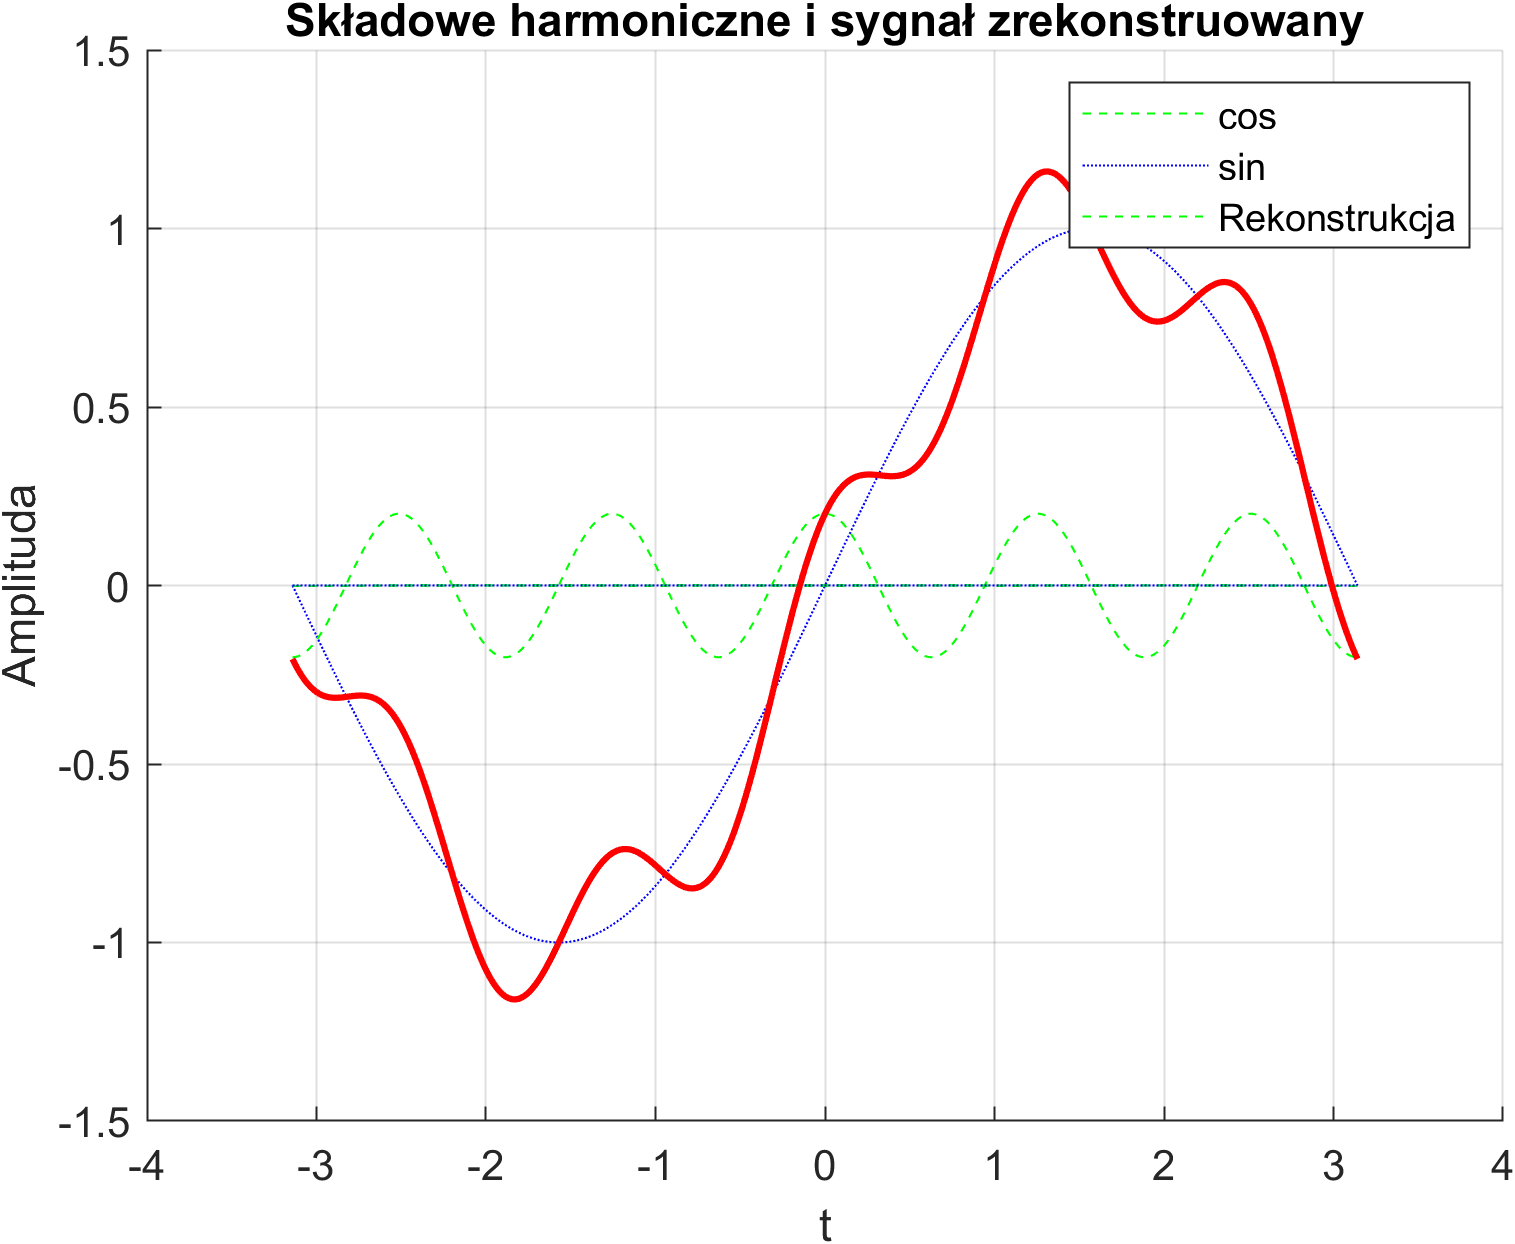
\includegraphics[width=\linewidth]{src/Lab005/recon_harmon.png}
		\label{fig:lab5z1_recon_harmon}
	\end{subfigure}
	\hfill
	\begin{subfigure}[t]{0.45\linewidth}
		\centering
		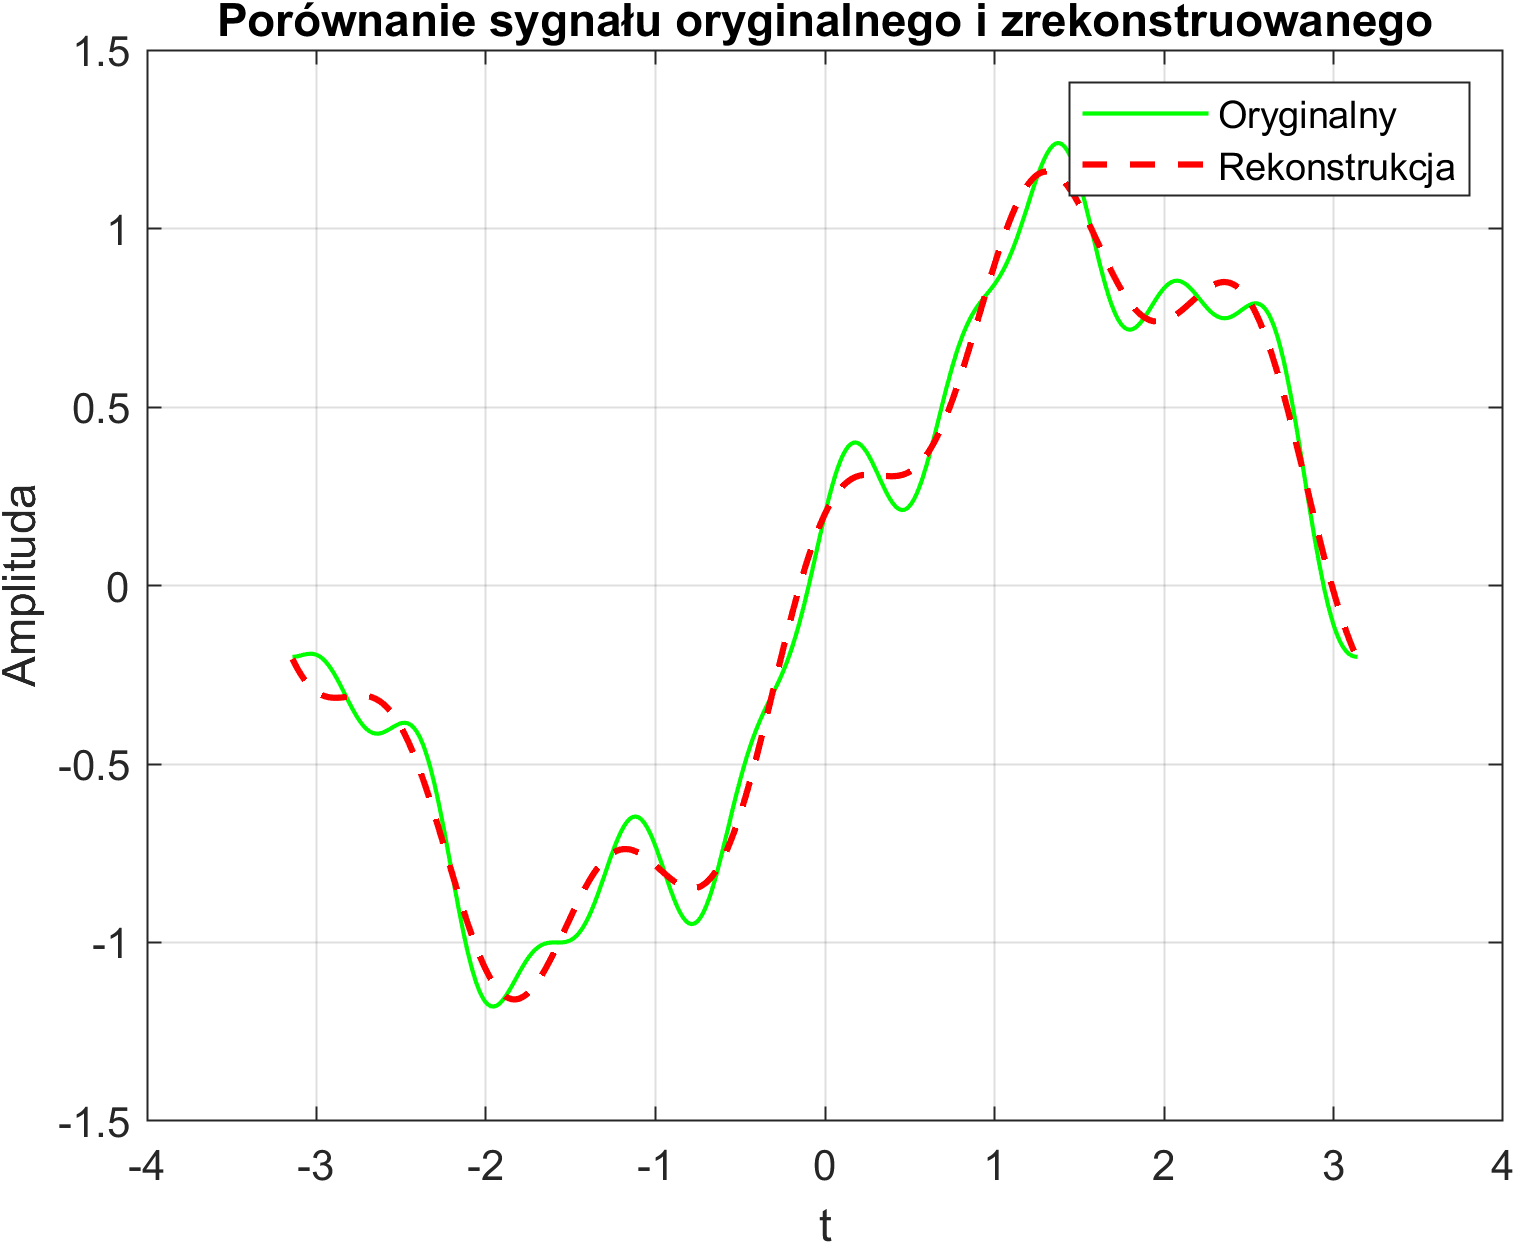
\includegraphics[width=\linewidth]{src/Lab005/comparison.png}
		\label{fig:lab5_comparison}
	\end{subfigure}
	
	\centering
	\begin{subfigure}[t]{0.45\linewidth}
		\centering
		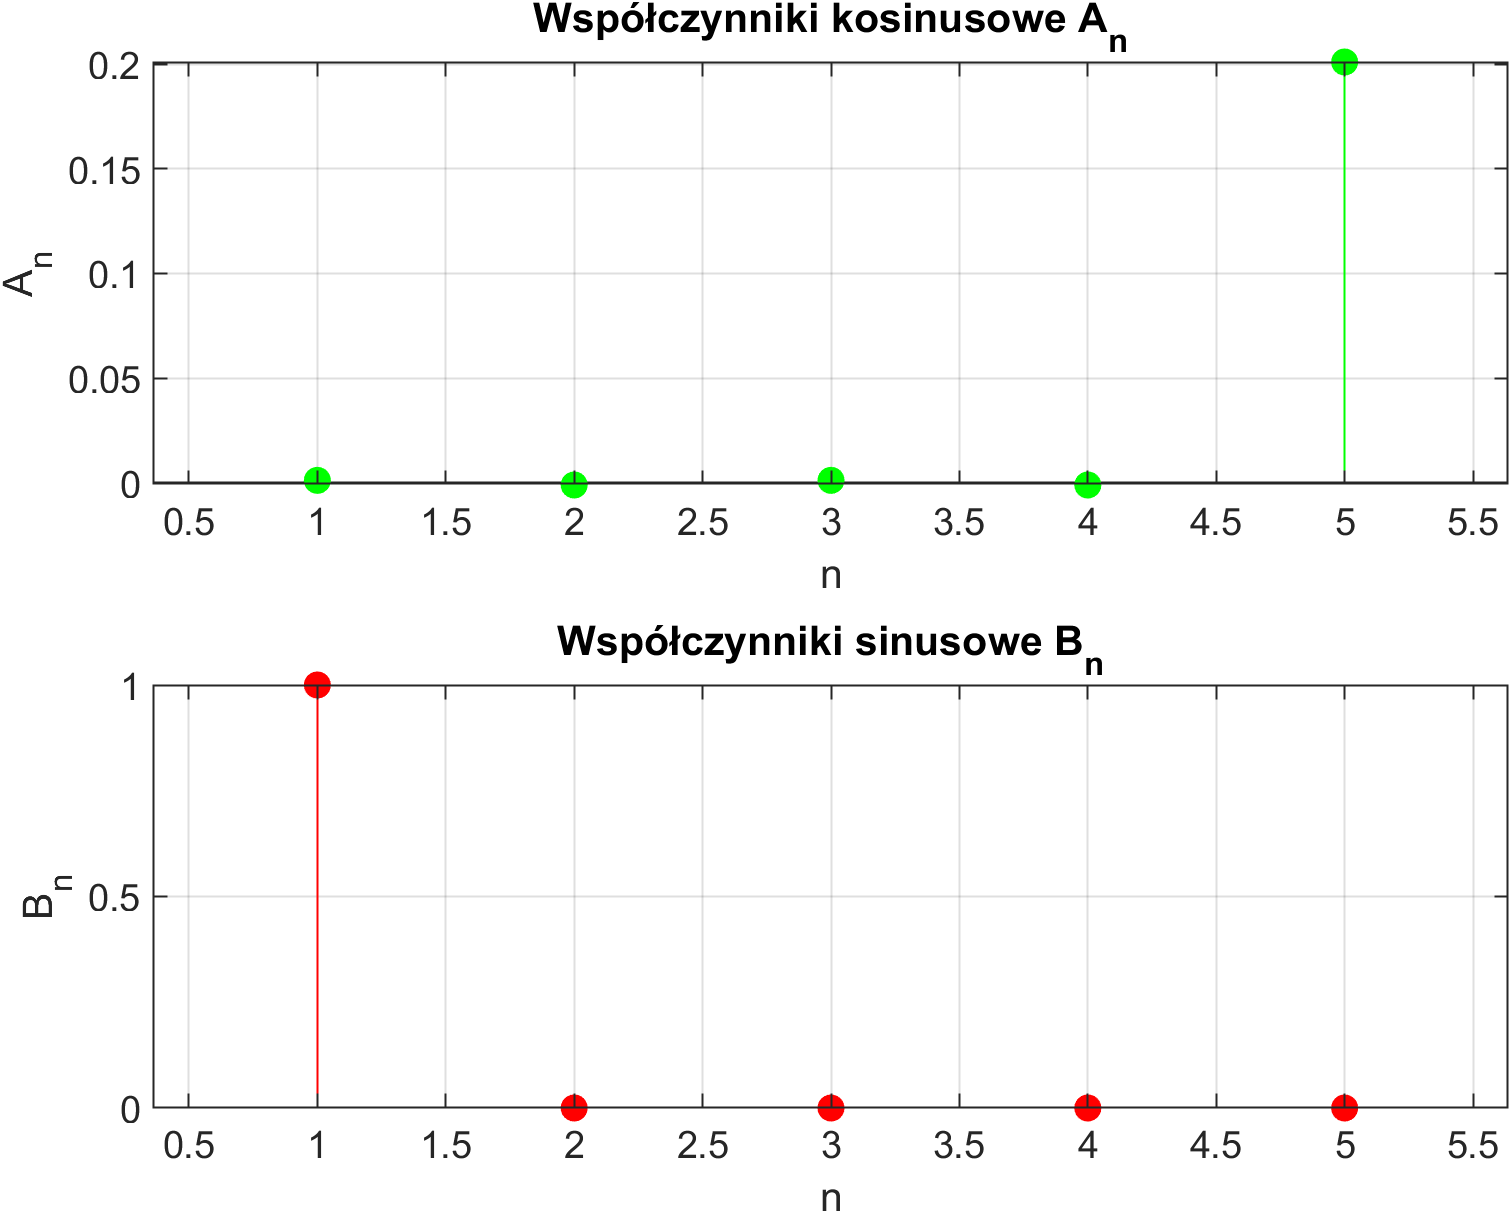
\includegraphics[width=\linewidth]{src/Lab005/coeff.png}
		\label{fig:lab5z1_coeff}
	\end{subfigure}
	\hfill
	\begin{subfigure}[t]{0.45\linewidth}
		\centering
		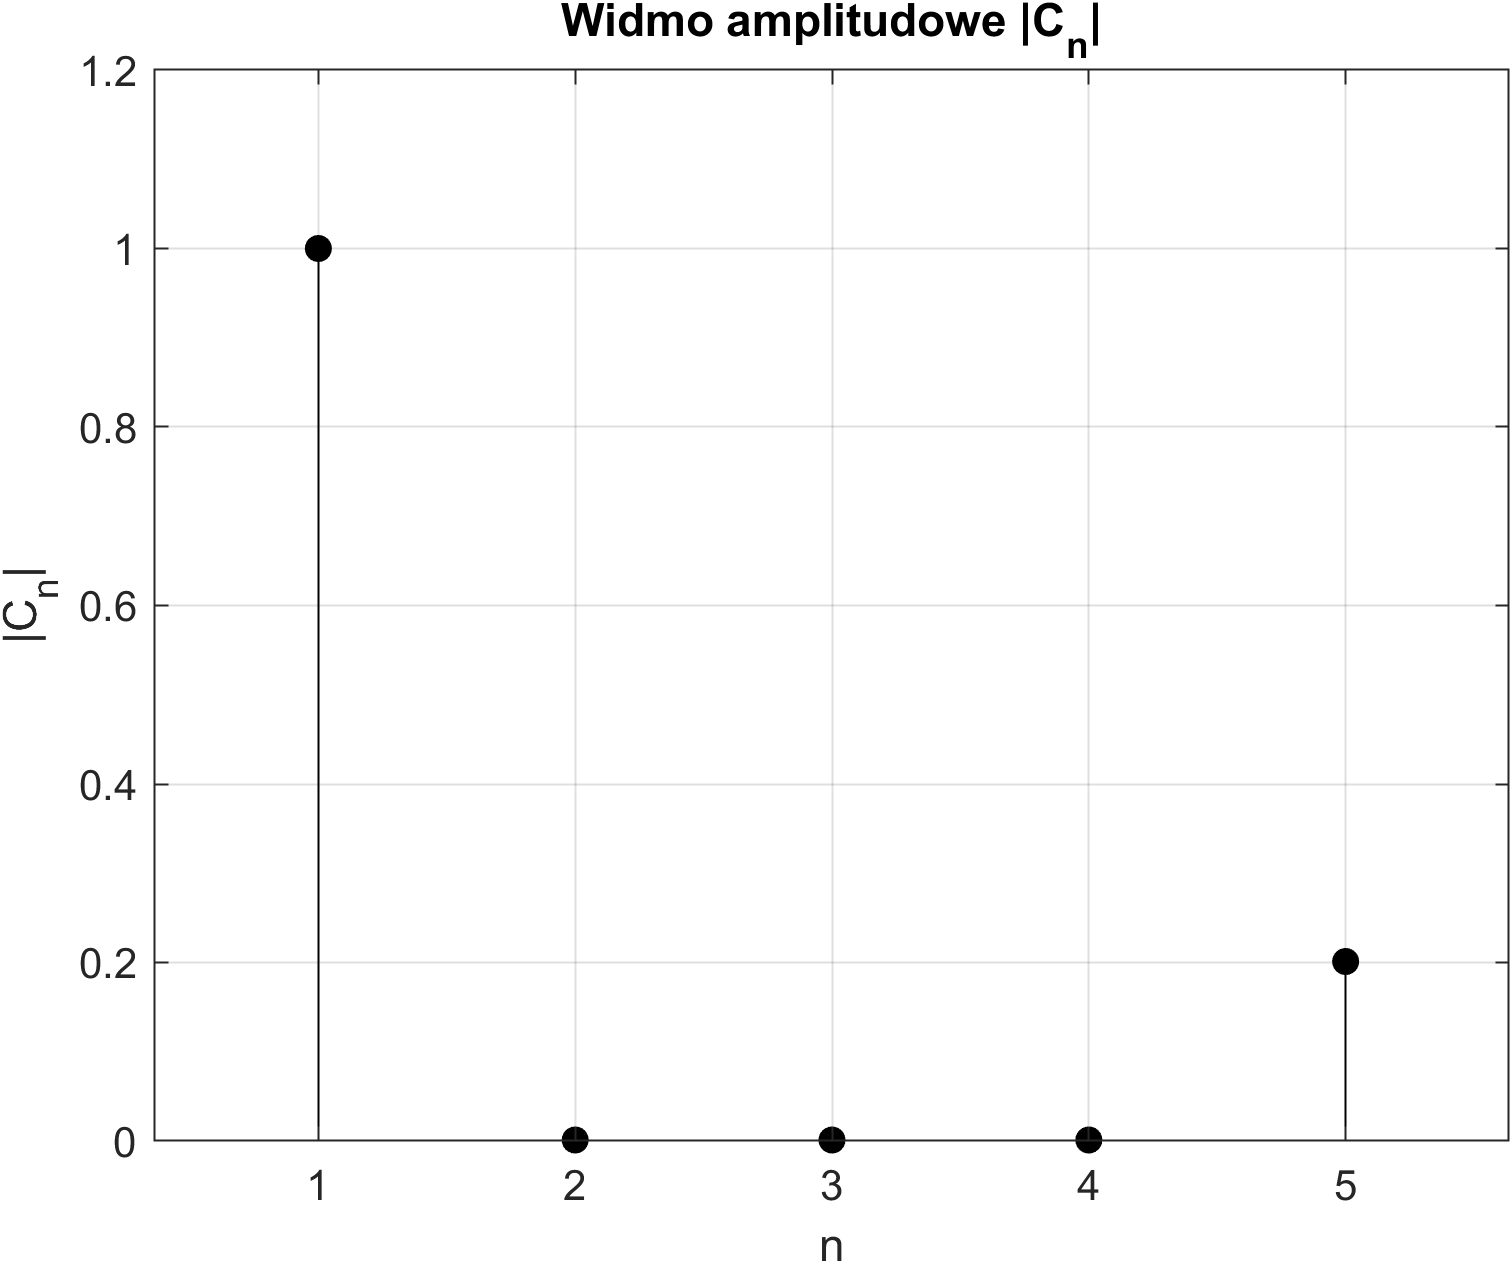
\includegraphics[width=\linewidth]{src/Lab005/spectrum.png}
		\label{fig:lab5_spectrum}
	\end{subfigure}
	\caption{Obrazy wyniku działania algorytmu rozkładu w szereg.}
\end{figure}

\subsection{Zadanie 2}

\subsubsection{Treść}

Wykorzystując dwuwymiarową transformatę Fouriera zaproponuj jego implementację oraz wykonaj
eksperymenty z filtracją środkowo przepustową obrazu tęczówki oka podanej przez prowadzącego.
Poniżej przedstawiono przykładowe rezultaty uzyskane dla obrazu Lena z wykorzystaniem maski
prostokątnej.

\subsubsection{Przykładowy program}

\lstinputlisting[style= matlabStyle, caption= Algorytm rozkładu w szereg Fouriera, label=Lab005_l2]{src/Lab005/zadanie2.m}

\subsubsection{Obrazy}

\begin{figure}[H]
	\centering
	\begin{subfigure}[t]{0.45\linewidth}
		\centering
		
\includegraphics[width=\linewidth]{src/lab005/zad2_iris_original.png}
		\label{fig:lab5z2_original}
	\end{subfigure}
	
	\centering
	\begin{subfigure}[t]{0.45\linewidth}
		\centering
		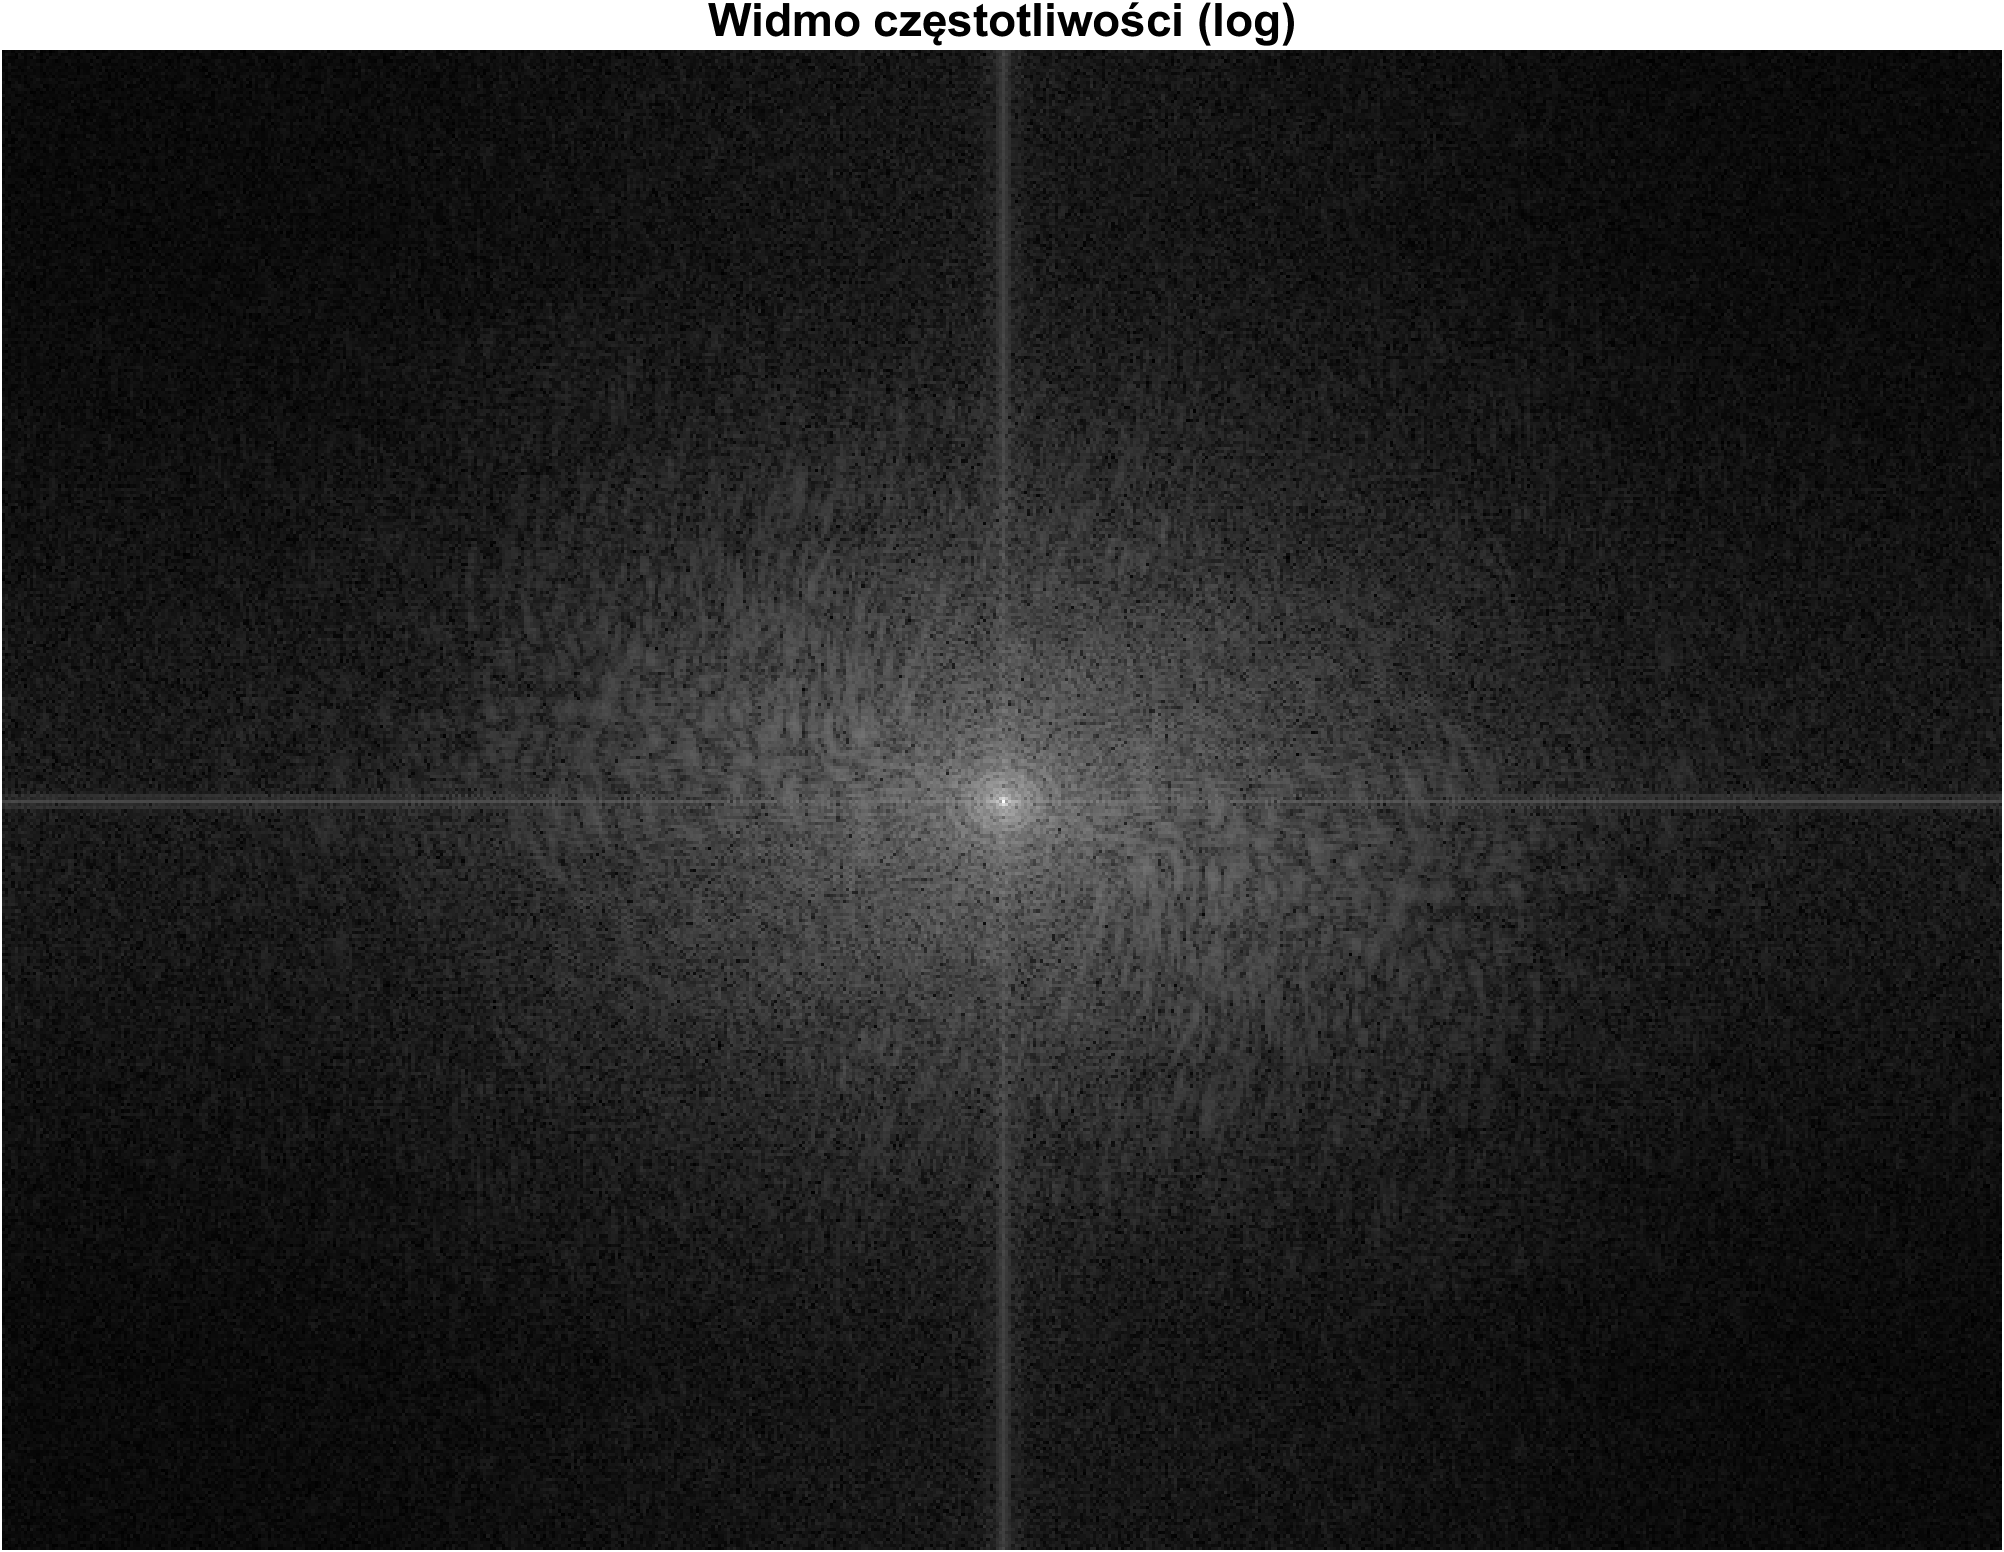
\includegraphics[width=\linewidth]{src/Lab005/zad2_iris_fft_spectrum.png}
		\label{fig:lab5z2_spectrum}
	\end{subfigure}
	\hfill
	\begin{subfigure}[t]{0.45\linewidth}
		\centering
		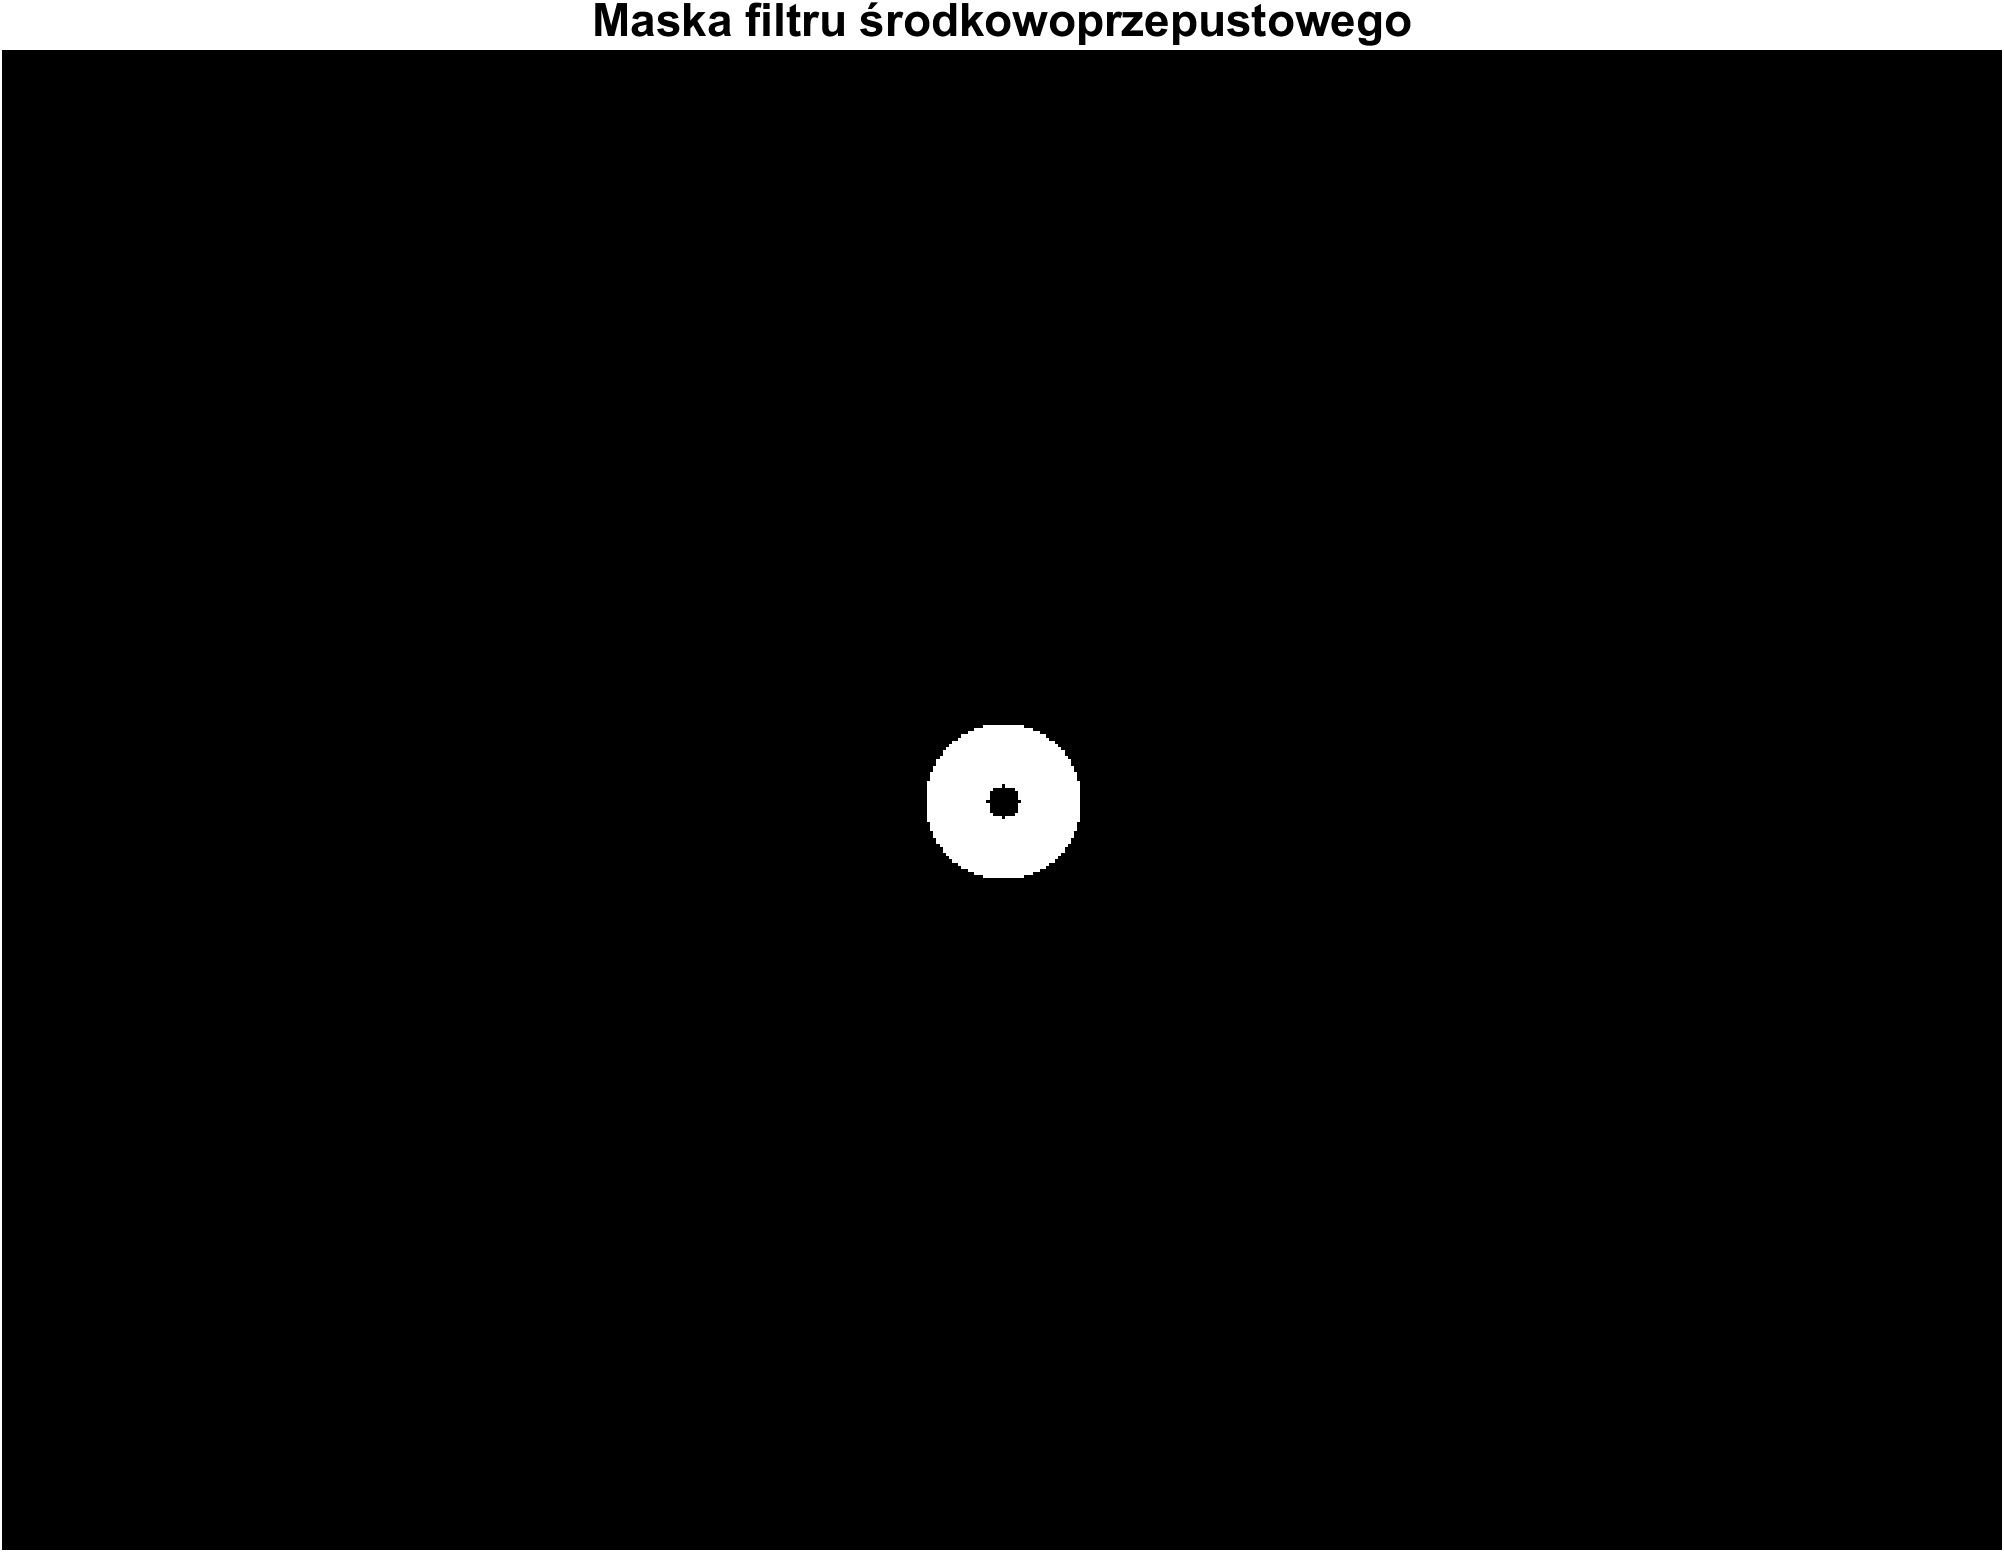
\includegraphics[width=\linewidth]{src/Lab005/zad2_iris_filter_mask.png}
		\label{fig:lab5z2_mask}
	\end{subfigure}
	
	\centering
	\begin{subfigure}[t]{0.45\linewidth}
		\centering
		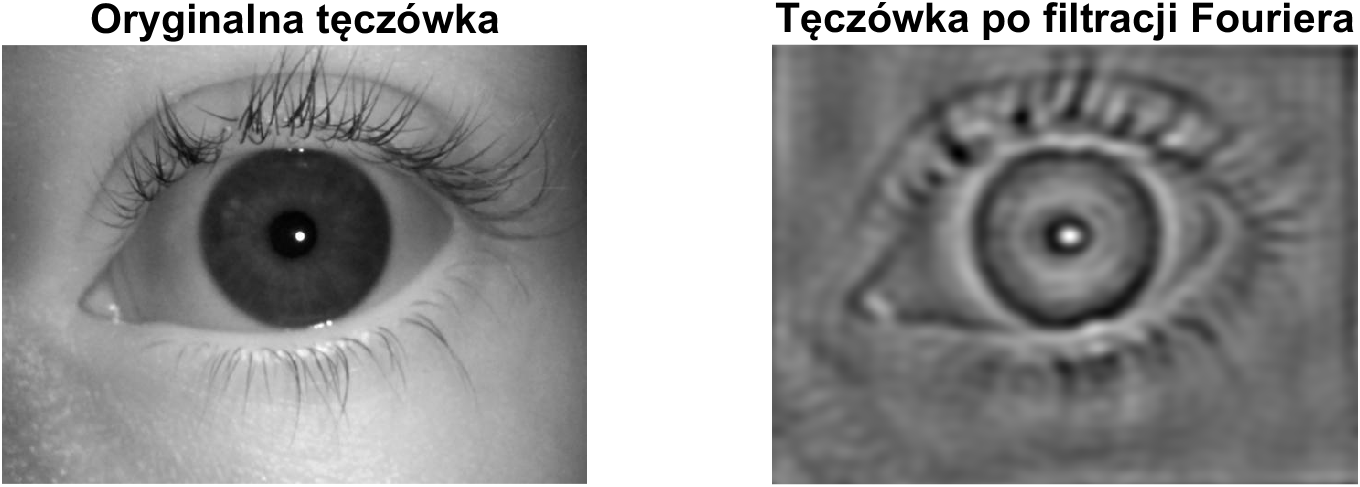
\includegraphics[width=\linewidth]{src/Lab005/zad2_iris_comparison.png}
		\label{fig:lab5z2_comparison}
	\end{subfigure}
	\hfill
	\begin{subfigure}[t]{0.45\linewidth}
		\centering
		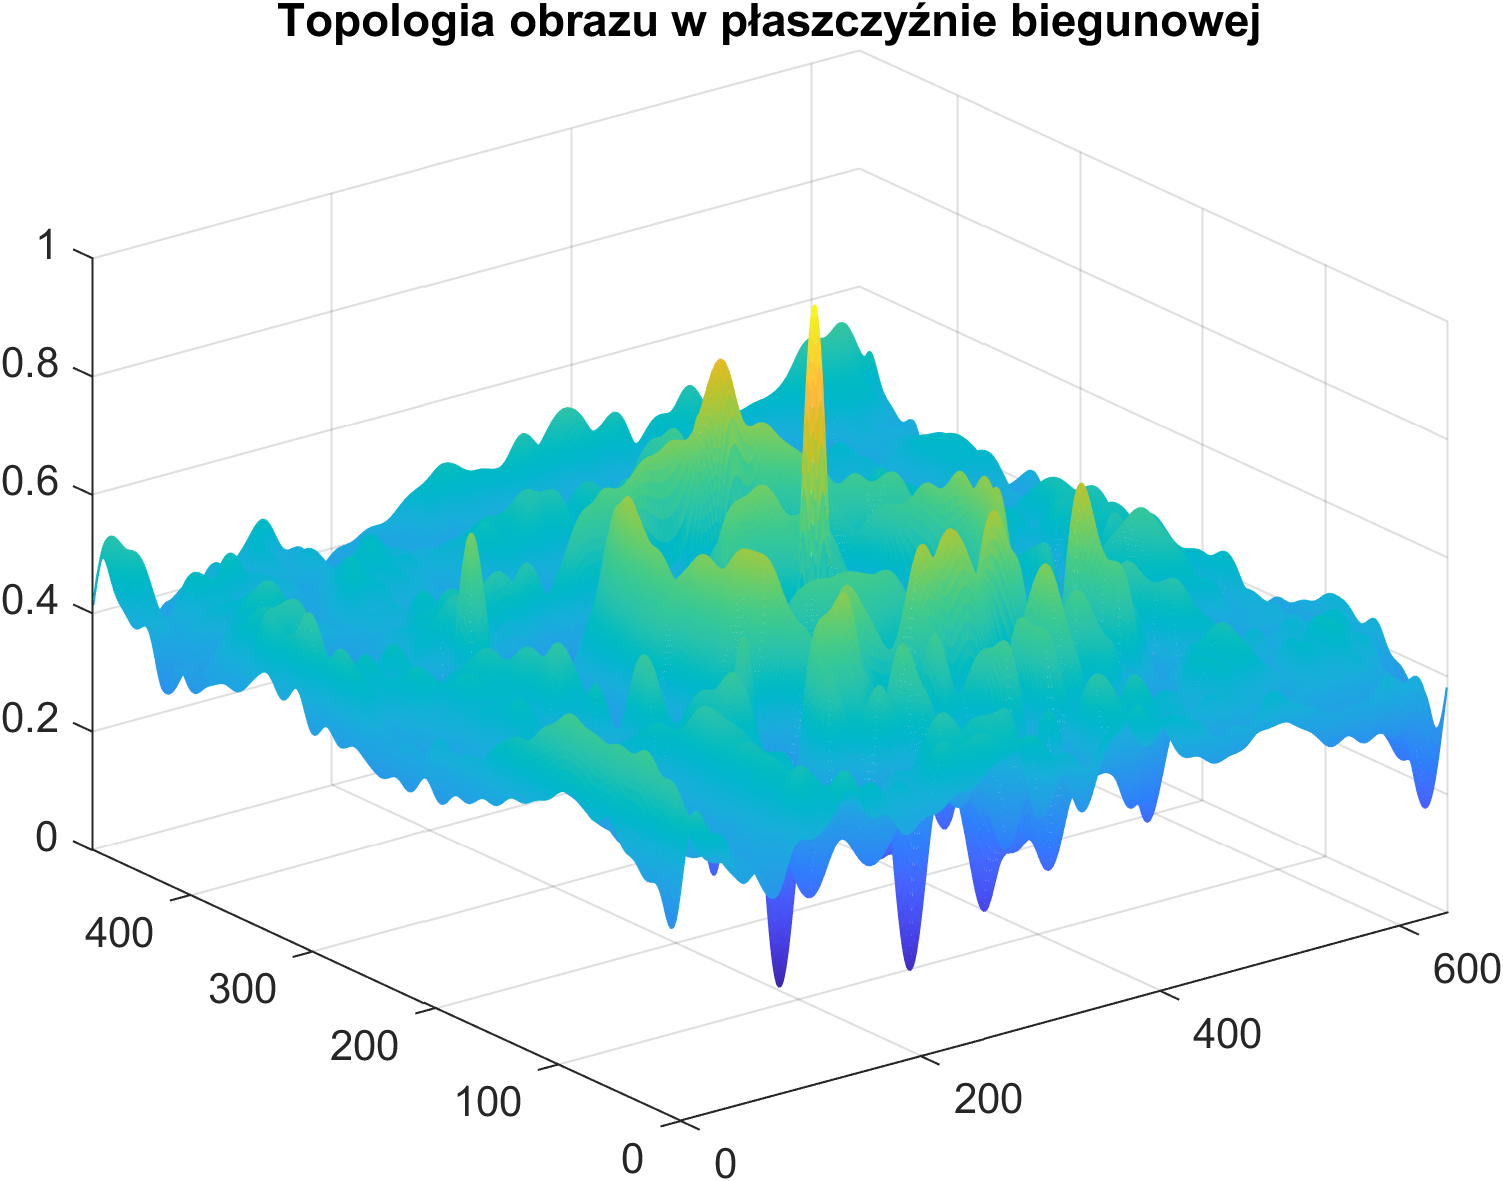
\includegraphics[width=\linewidth]{src/Lab005/zad2_iris_surface_plot.png}
		\label{fig:lab5_surface}
	\end{subfigure}
\end{figure}

\subsection{Zadanie 3}

\subsubsection{Treść}

Przetestuj przedstawiony powyżej mechanizm filtracji częstotliwościowej na obrazie
daktyloskopijnym.

\subsubsection{Przykładowy program}

\lstinputlisting[style= matlabStyle, caption= Algorytm rozkładu w szereg Fouriera, label=Lab005_l3]{src/Lab005/zadanie3.m}

\subsubsection{Obrazy}

\begin{figure}[H]
	\centering
	\begin{subfigure}[t]{0.45\linewidth}
		\centering
		
\includegraphics[width=\linewidth]{src/lab005/fingerprint_original.png}
		\label{fig:lab5z3_original}
	\end{subfigure}
	\hfill
	\begin{subfigure}[t]{0.45\linewidth}
		\centering
		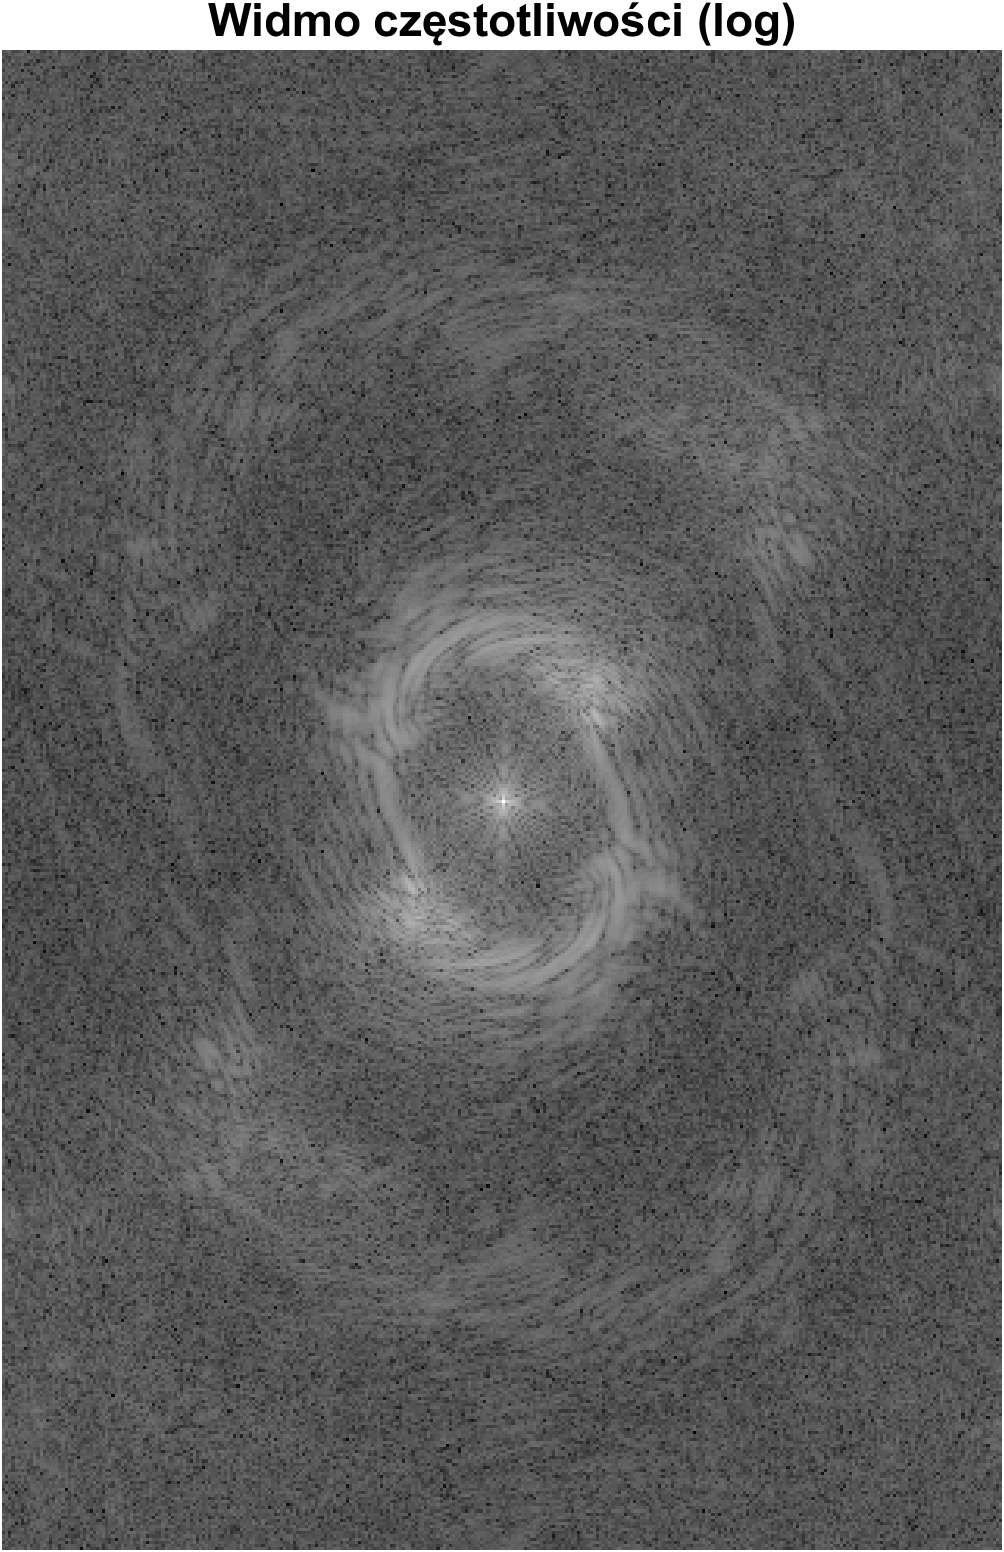
\includegraphics[width=\linewidth]{src/Lab005/fingerprint_fft_spectrum.png}
		\label{fig:lab5z3_spectrum}
	\end{subfigure}
	
	\centering
	\begin{subfigure}[t]{0.45\linewidth}
		\centering
		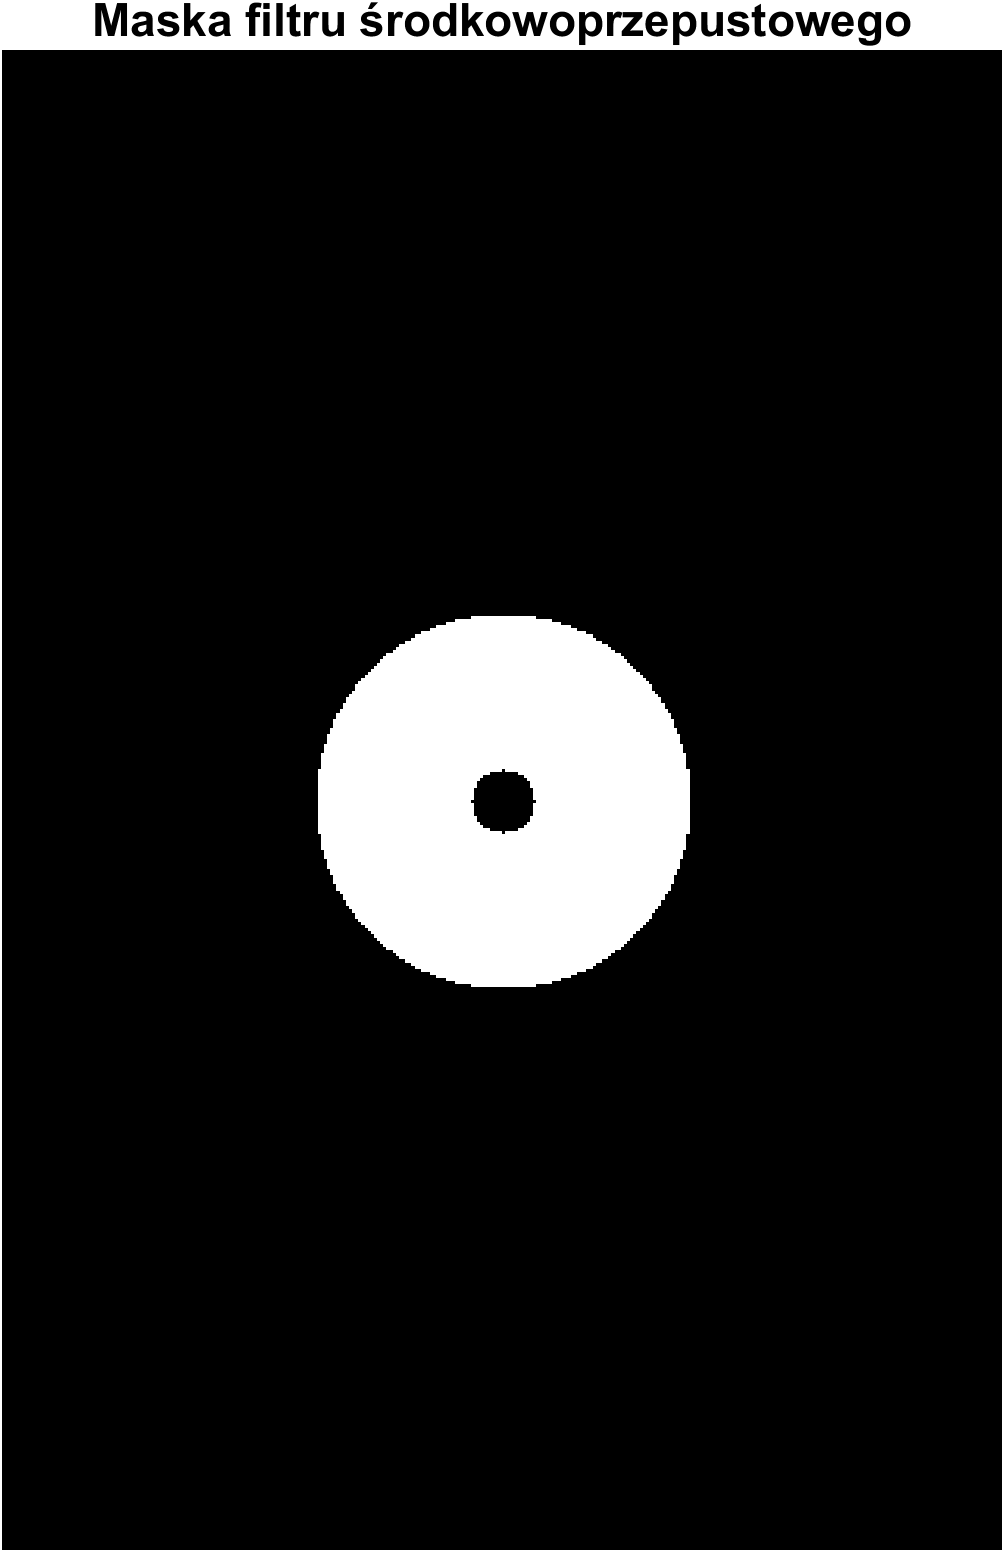
\includegraphics[width=\linewidth]{src/Lab005/fingerprint_filter_mask.png}
		\label{fig:labz3_mask}
	\end{subfigure}
	\hfill
	\begin{subfigure}[t]{0.45\linewidth}
		\centering
		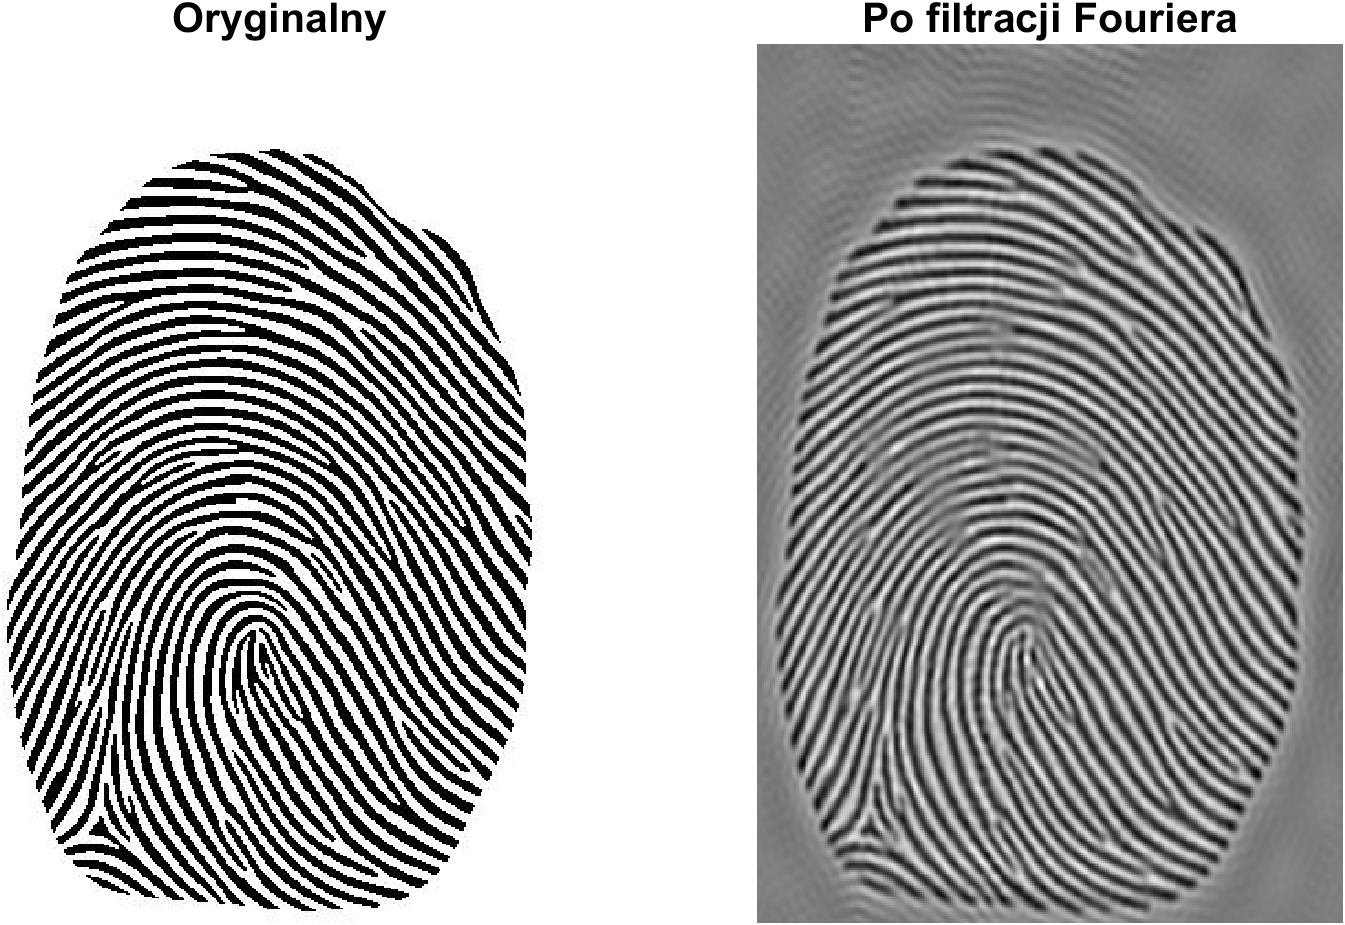
\includegraphics[width=\linewidth]{src/Lab005/fingerprint_comparison.png}
		\label{fig:lab5z3_comparison}
	\end{subfigure}
\end{figure}

\section{Wnioski}

Na podstawie przeprowadzonych eksperymentów można stwierdzić, że:

\subsection{Zadanie 1 – Szereg Fouriera dla sygnału okresowego}
\begin{itemize}
	\item Szereg Fouriera umożliwia rozkład złożonego sygnału okresowego na sumę składowych harmonicznych (sinusoidalnych).
	\item Liczba uwzględnionych harmonicznych (\texttt{roz}) znacząco wpływa na jakość rekonstrukcji – większa liczba pozwala dokładniej odwzorować kształt sygnału.
	\item Współczynniki $A_n$ i $B_n$ opisują odpowiednio składowe kosinusowe i sinusowe sygnału. Ich analiza pozwala zrozumieć udział poszczególnych częstotliwości.
	\item Rekonstrukcja sygnału z ograniczonej liczby harmonicznych jest skuteczna, lecz może prowadzić do efektu Gibbsa na nieciągłościach.
\end{itemize}

\subsection{Zadanie 2 – Filtracja obrazu tęczówki (2D FFT)}
\begin{itemize}
	\item Dwuwymiarowa transformata Fouriera pozwala analizować zawartość częstotliwościową obrazu i stosować filtry bezpośrednio w dziedzinie częstotliwości.
	\item Filtr środkowoprzepustowy skutecznie eliminuje zarówno niskie częstotliwości (np. niejednolite oświetlenie), jak i wysokie (szumy), pozostawiając najistotniejsze struktury tęczówki.
	\item Poprawiona zostaje czytelność wzorca tęczówki, co jest przydatne w systemach biometrycznych.
	\item Prosta maska w postaci pierścienia (idealny filtr pasmowy) jest łatwa do implementacji i daje dobre efekty wizualne.
\end{itemize}

\subsection{Zadanie 3 – Filtracja obrazu daktyloskopijnego (odcisk palca)}
\begin{itemize}
	\item Obraz odcisku palca również można skutecznie analizować i przetwarzać w dziedzinie częstotliwości przy użyciu 2D FFT.
	\item Filtracja środkowoprzepustowa umożliwia eliminację tła i szumów, wzmacniając jednocześnie struktury grzbietów i bruzd.
	\item Wynikowy obraz po filtracji zawiera bardziej wyraziste cechy, co ułatwia dalsze etapy przetwarzania, takie jak wykrywanie minutiae.
	\item Odpowiedni dobór zakresu częstotliwości w masce filtru ma kluczowe znaczenie dla jakości uzyskanego obrazu.
\end{itemize}


